\documentclass[12pt]{article}
\usepackage{pgf, tikz}
\usepackage{amsmath, amsfonts, amssymb, graphicx}
\usepackage{float}
\usepackage{subfig}
\usepackage[utf8]{inputenc}
\usepackage[spanish]{babel}
\usepackage{amsthm}
\usepackage{caption}

\setlength{\textheight}{23cm} \setlength{\evensidemargin}{0cm}
\setlength{\oddsidemargin}{-.5cm} \setlength{\topmargin}{-3cm}
\setlength{\textwidth}{17.5cm} \setlength{\parskip}{.2cm}


%opening

\begin{document}
	\begin{picture}(80, 80)
	\put(170,0){\hbox{
\includegraphics[scale=0.6]{cimat_logo.png}}}
	\end{picture}
	
	\begin{center}
		\begin{huge}
			Centro de Investigación en Matemáticas, A.C.
		\end{huge}
	\end{center}

	\begin{center}
		\begin{large}
			Descripción tarea 11 - Métodos numéricos
		\end{large}
	\end{center}
	
	\begin{center}
		\textbf{Erick Salvador Alvarez Valencia}
	\end{center}

	\begin{center}
		9 de Noviembre de 2017
	\end{center}



%\maketitle

%\tableofcontents

\section{Introducción}
En el presente reporte se describirán los resultados obtenidos del método de Romberg el cual se usa para calcular la integral definida de una función contínua. Dicho algoritmo emplea internamente el método recursivo del trapecio y la extrapolación de Richardson para mejorar la aproximación de la integral. Para concluir se mostrarán algunos ejemplos de ejecuciones realizadas con diversas funciones y diferente número de particiones.

\section{Descripción}
Como se mencionó anteriormente, un método numérico para calcular la integral de una función continua es el del trapecio, el cual realiza se basa en hacer una interpolación con un polinomio de grado 1 el cual pasará por dos puntos, de ahí se podrá notar que se tiene la forma de un trapecio la cual su área se aproximará al área bajo la curva de la función. Su fórmula es la siguiente:

$$\int_{a}^{b}f(x) dx \approx h [\frac{f(a) + f(b)}{2} + \sum_{i=1}^{n - 1}f(x_i)]$$

donde $h = \frac{(b - a)}{n}$. La formula anterior refiere al método del trapecio definido a pedazos, la idea es generar una partición uniforme dentro del rango $[a, b]$ y para cada par de puntos aplicar el método, esto mejorará la aproximación del área.\\

La regla recursiva del trapecio es una mejora que nos permite usar lo anterior para calcular la integral sin tener que evaluar la función en puntos previamente evaluados. En general la regla nos dice que:\\

$R(n, 0) = \frac{b - a}{2}[f(a) + f(b)]$ si $n = 0$ y $R(n, 0) = \frac{h}{2}[f(a) + f(b)] + h \sum_{i = 1}^{2^n - 1} f(a + ih)$ si $n > 0$\\

La extrapolación de Richardson permite construir a partir de una secuencia convergente otra secuencia más rápidamente convergente. Esta técnica se usa frecuentemente para mejorar los resultados de métodos numéricos a partir de una estimación previa, en este caso la usaremos para definir el método de Romberg el cual evalúa el integrando en puntos equiespaciados del intervalo de integración estudiado. Para que este método funcione, el integrando debe ser suficientemente derivable en el intervalo, aunque se obtienen resultados bastante buenos incluso para integrandos poco derivables.\\
El método se crea de forma recursiva usando la definición anterior dada con la regla del trapecio, dicha fórmula nos permite calcular los valores de la primer columna. Ahora para obtener los valores de las siguientes se usan los de la columna previamente calculada usando lo siguiente:

$$R(n, m) = R(n, m - 1) + \frac{1}{4^m - 1}[R(n, m - 1) - R(n - 1, m - 1)]$$

Calculamos recursivamente hasta tener el valor de R(n, n) el cual será la mejor aproximación que este método nos dará.

\section{Ejemplo de ejecución}
El algoritmo se probó con varias funciones diferenciables y nos brindó muy buenos resultados, para el presente se mostrarán en particular contra las funciones $f_1(x) = sin(2 \pi x)$ y $f_2(x) = 4x^3 - 2x + 1$ y con diferentes valores de $n$.

\begin{figure}[H]
	\centering
	\subfloat[][Figura 1. Resultados para ejecución función 1, n = 4.]{
		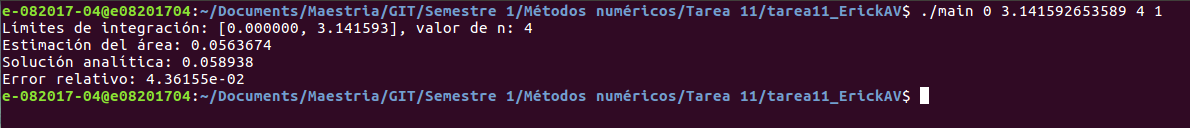
\includegraphics[scale=0.3]{E41.png}
	}\hfill
\end{figure}

\begin{figure}[H]
	\centering
	\subfloat[][Figura 2. Resultados para ejecución función 1, n = 6.]{
		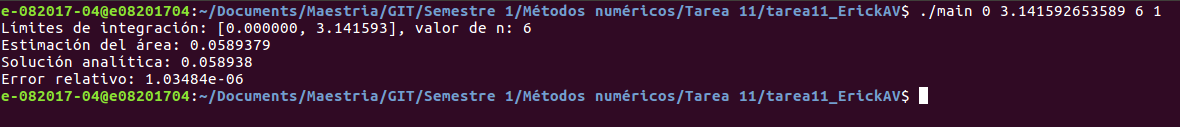
\includegraphics[scale=0.3]{E61.png}
	}\hfill
\end{figure}

\begin{figure}[H]
	\centering
	\subfloat[][Figura 3. Resultados para ejecución función 1, n = 8.]{
		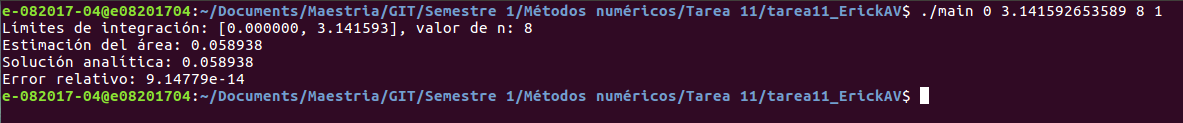
\includegraphics[scale=0.3]{E81.png}
	}\hfill
\end{figure}

Podemos ver en las imágenes anteriores que el resultado mejora bastante únicamente con un pequeño aumento en las particiones.

\begin{figure}[H]
	\centering
	\subfloat[][Figura 4. Resultados para ejecución función 2, $n$ = 4.]{
		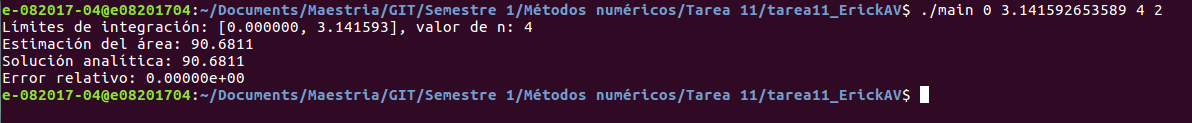
\includegraphics[scale=0.3]{E42.png}
	}\hfill
\end{figure}

\begin{figure}[H]
	\centering
	\subfloat[][Figura 5. Resultados para ejecución función 2, $n$ = 6.]{
		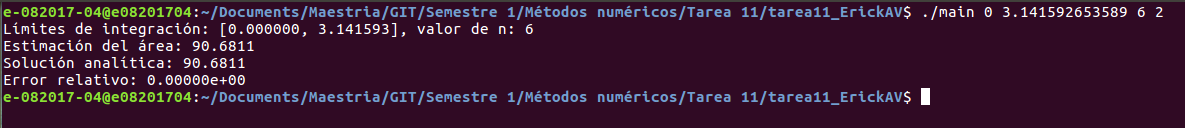
\includegraphics[scale=0.3]{E62.png}
	}\hfill
\end{figure}

\begin{figure}[H]
	\centering
	\subfloat[][Figura 6. Resultados para ejecución función 2, $n$ = 8.]{
		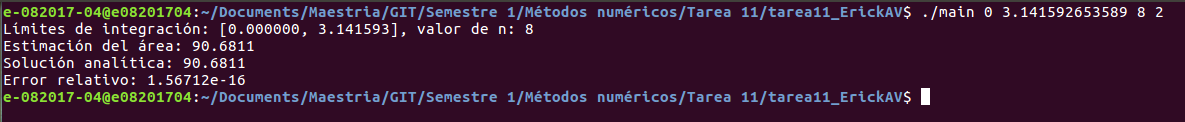
\includegraphics[scale=0.3]{E82.png}
	}\hfill
\end{figure}

Podemos ver en las tres imágenes anteriores desde que el valor de $n$ es 4 ya tenemos la aproximación exacta (o casi exacta) del área bajo la curva.

\section{Compilación y ejecución}
\textbf{Para compilar:} En la carpeta encontraremos los archivos $.c$ y $.h$ con los que se podrá compilar el ejecutable. De la misma forma, en conjunto con los archivos anteriores, también podremos encontrar un Makefile para, en caso de encontrarse en linux, compilar de manera sencilla.

\begin{enumerate}
	\item \textbf{Compilar usando Makefile:} En la terminal, nos colocamos en el directorio donde se encuentre el programa, y ejecutamos el comando $make$, automáticamente se realizará la compilación y se generará el ejecutable. El Makefile también contiene el comando $make\ clean$ el cual limpiará los archivos generados por la compilación, incluyendo el ejecutable.
	\item \textbf{Compilar directamente:} De la misma forma, podemos compilar directamente usando los siguientes comandos (en terminal):
	\begin{itemize}
		\item gcc -c main.c -o obj/main.o
		\item gcc -c memo.c -o obj/memo.o
		\item gcc -c met\_num.c -o obj/met\_num.o
		\item gcc -o main obj/main.o obj/memo.o obj/met\_num.o\ -lm
	\end{itemize}
\end{enumerate}

\textbf{Para ejecutar:} Únicamente debemos de usar el comando $./main$ para ejecutar el programa en consola, este recibe los siguientes argumentos:
\begin{itemize}
	\item \textbf{Un número decimal:} El límite inferior del intervalo.
	\item \textbf{Un número decimal:} El límite superior del intervalo.
	\item \textbf{Un entero:} El número de particiones.
	\item \textbf{Un entero:} El tipo de función que se usará (función 1 o función 2). 
\end{itemize}

El programa ejecutará el método de Romberg para la función y límites indicados, al final imprimirá el valor del área estimado, el área obtenida con la expresión analítica y el error relativo.\\

\textbf{Ejemplo de ejecución:} ./main 0 3.141592653589 8 2\\

Ahí estamos diciendo que los límites de integración van de 0 a $\pi$, que queremos una partición de $n = 8$ y que usaremos la función 2.\\
Las funciones que tiene el código son las siguientes:
\begin{enumerate}
	\item $f(x) = sin(2 \pi x)$
	\item $f(x) = 4x^3 - 2x + 1$
\end{enumerate}

\end{document}
